%%%%%%%%%%%%%%%%%%%%%%%%%%%%%%%%%%%%% 
%% LE2I beamer template
%% Guillaume Lemaitre, October 2014
%%%%%%%%%%%%%%%%%%%%%%%%%%%%%%%%%%%%% 

\documentclass[table]{beamer}

\usepackage[utf8]{inputenc}
\usepackage[T1]{fontenc} 
\usetheme{le2i} 

%% The amssymb package provides various useful mathematical symbols
\usepackage{amssymb}
%% The amsthm package provides extended theorem environments
\usepackage{amsthm}
%% amsmath for math environment
\usepackage{amsmath}

\DeclareMathOperator*{\argmin}{arg\,min}
\DeclareMathOperator*{\argmax}{arg\,max}
\DeclareMathOperator*{\sign}{sign}

%% figure package
\usepackage{epsf,graphicx}
\usepackage{epstopdf}
\usepackage{subfigure}
\usepackage{transparent}
\usepackage{fixltx2e}

%% In order to draw some graphs
\usepackage{tikz,xifthen}
\usepackage{tikz-qtree}
\usepackage{adjustbox}
\usetikzlibrary{decorations.pathmorphing}
\usetikzlibrary{fit}
\usetikzlibrary{backgrounds}
\usetikzlibrary{shapes,arrows,shadows}
\usetikzlibrary{calc,decorations.pathreplacing,decorations.markings,positioning}
\usetikzlibrary{snakes,decorations.text,shapes,patterns}
% \usepackage{scalefnt,lmodern,booktabs}

%% Package for cross and tick symbols
\usepackage{pifont}
\newcommand{\tick}{\color{green!60!black!80}\ding{51}}
\newcommand{\cross}{\color{red!60!black!80}\ding{55}}

%\usepackage[table]{xcolor}

\title{Introduction to Image Processing}
\author{Guillaume Lema\^itre \\ \texttt{guillaume.lemaitre@udg.edu}}
\date{Lecture 1 \\ 16\textsuperscript{th} Sept. 2015}

\institute{Universit\'e de Bourgogne} 

%% Uncomment if you want to avoid thousand of bullet inside the menu
% \usepackage{etoolbox}
% \makeatletter
% \patchcmd{\slideentry}{\advance\beamer@xpos by1\relax}{}{}{}
% \def\beamer@subsectionentry#1#2#3#4#5{\advance\beamer@xpos by1\relax}%
% \makeatother

\begin{document}

% Show the title page
\begin{frame}
  \titlepage
\end{frame}

% Show the table of contents
\begin{frame}
  \tableofcontents[sectionstyle=show,subsectionstyle=show,subsubsectionstyle=hide]
\end{frame}

\section{Human Vision}

\subsection{Human eye}

\begin{frame}
  \frametitle{Human Vision}
  \framesubtitle{Human eye}
  \begin{block}{From the eye to a camera}
    \begin{columns}
      \begin{column}{.5\linewidth}
        \begin{center}
          \only<1>{Choroid}
          \only<2>{Ciliary body \& iris}
          \only<3>{Lens}
          \only<4>{Retina}
          \only<5>{Cones}
          \only<6>{Rods}
          \only<7>{Cones \& Rods}
          \only<8>{Fovea}
        \end{center}
        \begin{itemize}\scriptsize
          \only<1>{\item Composed of blood vessels serving as source of nutrition
          \item Avoid the entrance of external light or backscatter
          \item See relation with physics experiments}
          \only<2>{\item Control the amount of light (2 mm to 8 mm)
          \item Relation with the camera aperture}
          \only<3>{\item Made of fibrous cells and attached to ciliary body
          \item Absorb 8 \% of visible light and all the IR and UV
          \item Cataract diseases
          \item Idem to an optical lens}
          \only<4>{\item Contains 2 types of discrete light receptors: the cones and the rods
          \item Myopia \& hyperopia}
          \only<5>{\item Account for about 6 to 7 million per eye
          \item Are sensitive to color and details
          \item Each one connected to a single nerve end
          \item Cone vision is called \emph{photopic} and is sensitive to high levels of illumination
          \item Similar to a high frequency receptor}
          \only<6>{\item Account for 75 to 150 millions per eye
          \item Not involved in color
          \item Give a general and overall picture of the FOV
          \item Several rods connected to a single nerve end
          \item Sensitive to low levels of illuminations: \emph{scotopic}
          \item Similar to a low frequency receptor}
          \only<7>{\item Symmetrically distributed
          \item Note the presence of the blind spot}
          \only<8>{\item Localisation of the cones in this area
          \item 1.5 mm $\times$ 1.5 mm
          \item 150,000 elts/mm\textsuperscript{2} to 337,000 elts/mm\textsuperscript{2}
          \item CCD imaging ship would need a 5 mm $\times$ 5 mm to achieve similar density}
        \end{itemize}
      \end{column}
      \begin{column}{.5\linewidth}
        \only<1-6>{\begin{figure}
            \centering
            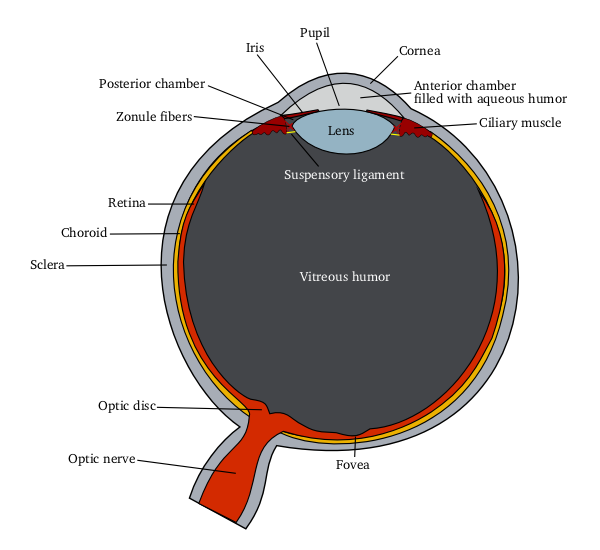
\includegraphics[width=.9\textwidth]{./images/eye.png}
          \end{figure}}
        \only<7>{\begin{figure}
            \centering
            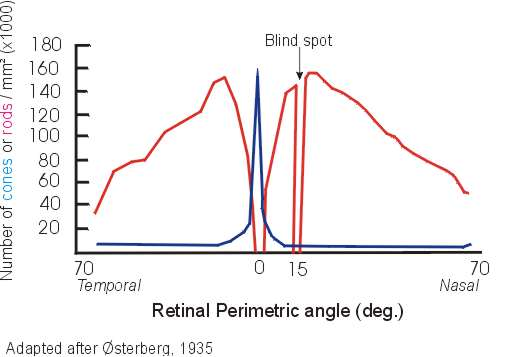
\includegraphics[width=.9\textwidth]{./images/distri.jpg}
          \end{figure}}
        \only<8>{\begin{figure}
            \centering
            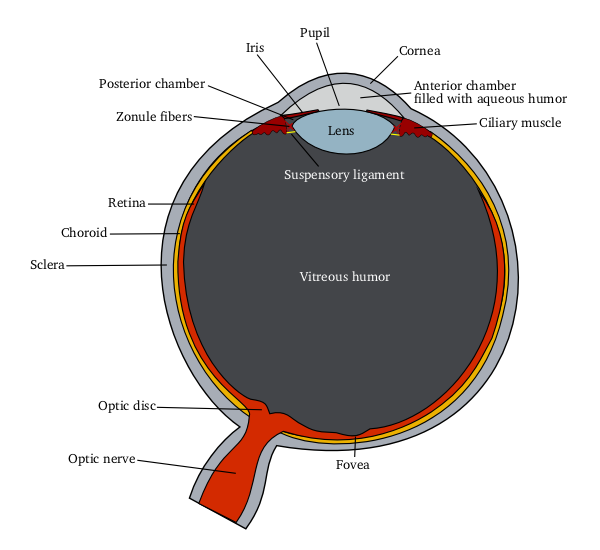
\includegraphics[width=.9\textwidth]{./images/eye.png}
          \end{figure}}
      \end{column}
    \end{columns}    
  \end{block}
\end{frame}

\subsection{Image formation in the eye}

\begin{frame}
  \frametitle{Human Vision}
  \framesubtitle{Image formation in the eye}
  \begin{block}{Example}
    \begin{figure}
      \centering
      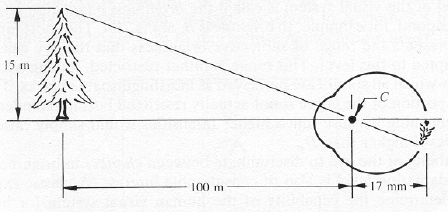
\includegraphics[width=.7\textwidth]{./images/form.png}
    \end{figure}
    \begin{itemize}\scriptsize
    \item Focal length varies from 17 mm to 14 mm
    \item Perception takes place by the relative excitation of light receptors.
    \item The receptors transform this energy to electrical impulses
    \end{itemize}
  \end{block}
\end{frame}

\subsection{Brightness adaptation \& discrimination}

\begin{frame}
  \frametitle{Human Vision}
  \framesubtitle{Brightness adaptation \& discrimination}
  \begin{block}{Human visual system}
    \begin{itemize}\scriptsize
    \item The human vision system (HVS) can adapt to $10^{10}$ light intensity levels
    \item Subjective brightness is a logarithmic function of the light intensity incident on the eye
      \begin{figure}
        \centering
        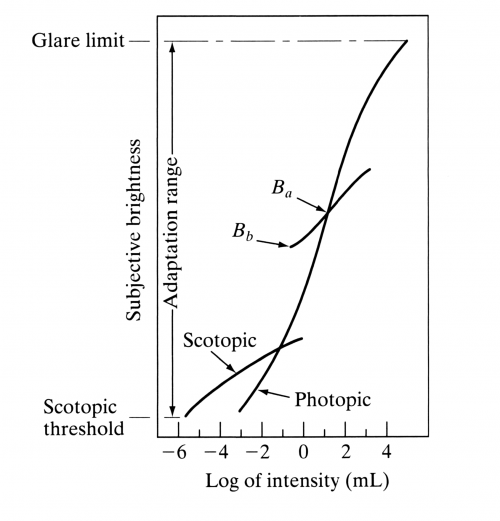
\includegraphics[height=.35\textheight]{./images/sb.png}
      \end{figure}
    \item The HVS cannot operate over such a range simultaneously
    \item For a given set of conditions, the current sensitivity level is called \emph{brightness adaptation level}
    \end{itemize}
  \end{block}
\end{frame}

\begin{frame}
  \frametitle{Human Vision}
  \framesubtitle{Brightness adaptation \& discrimination}
  \begin{block}{Human visual system}
    \begin{itemize}\scriptsize
    \item The eye also discriminates between changes in brightness at any specific adaption level
    \item This is characterised by the Weber ratio
    \end{itemize}
    \begin{equation}
      \frac{\Delta I_c}{I},
    \end{equation}
    {\scriptsize where $\Delta I_c$ is the increment of illumination discriminable 50 \% of the time and $I$ is the background illumination}
  \end{block}
\end{frame}

\begin{frame}
  \frametitle{Human Vision}
  \framesubtitle{Brightness adaptation \& discrimination}
  \begin{block}{Human visual system}
    \begin{figure}
      \centering
      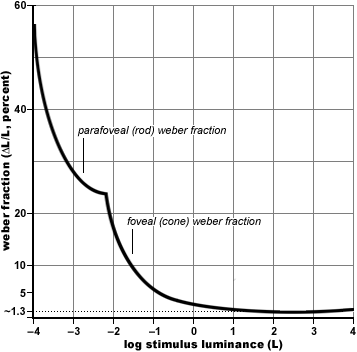
\includegraphics[height=.35\textheight]{./images/wr.png}
    \end{figure}
    \begin{itemize}\scriptsize
    \item Small values of Weber ration mean good brightness discrimination and vice versa
    \item At low levels of illumination brightness discrimination is poor (rods)
    \item It improves significantly as background illumination increases (cones)
    \item The typical observer can discern one to two dozen different intensity changes
    \end{itemize}
  \end{block}
\end{frame}

\begin{frame}
  \frametitle{Human Vision}
  \framesubtitle{Brightness adaptation \& discrimination}
  \begin{block}{Human visual system}
    \begin{itemize}\scriptsize
    \item Overall intensity discrimination is broad due to different set of incremental changes to be detected at each new adaptation level
    \item Perceived brightness is not a simple function of intensity: Mach band effect, simultaneously contrast, and optical effect
    \end{itemize}
  \end{block}
\end{frame}

\begin{frame}
  \frametitle{Human Vision}
  \framesubtitle{Brightness adaptation \& discrimination}
    \only<1>{\begin{block}{Mach band effect}
        \begin{figure}
        \centering
        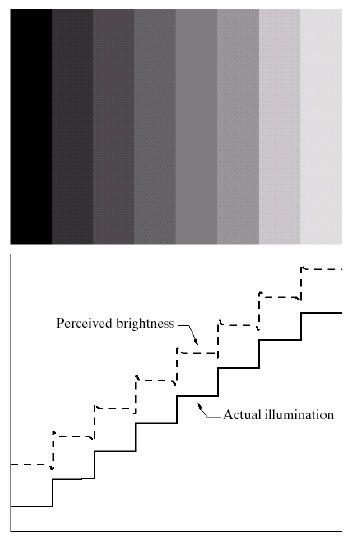
\includegraphics[height=.6\textheight]{./images/mach.png}
      \end{figure}
    \end{block}}
  \only<2>{\begin{block}{Simultaneously contrast}
        \begin{figure}
        \centering
        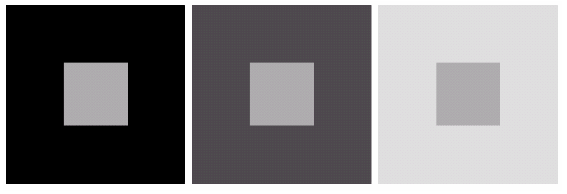
\includegraphics[width=.8\textwidth]{./images/sc.png}
      \end{figure}
    \end{block}}
  \only<3>{\begin{block}{Optical effect}
        \begin{figure}
        \centering
        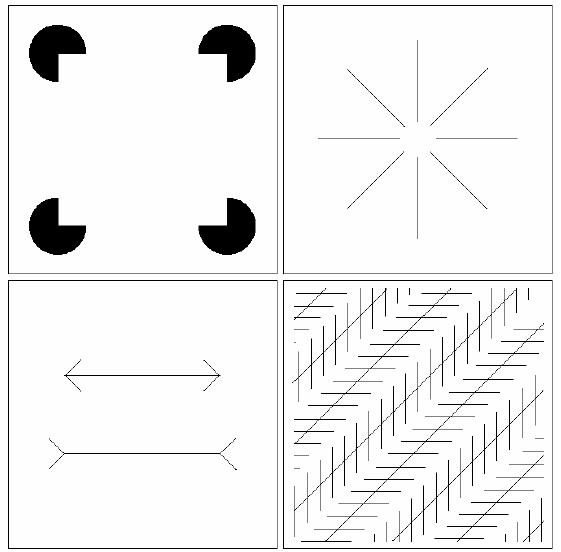
\includegraphics[height=.6\textheight]{./images/oe.png}
      \end{figure}
    \end{block}}
\end{frame}

\section{Digital Image}
\subsection{Formation}

\begin{frame}
  \frametitle{Digital Image}
  %\framesubtitle{}
    \begin{block}{Digital image formation}
        \begin{figure}
        \centering
        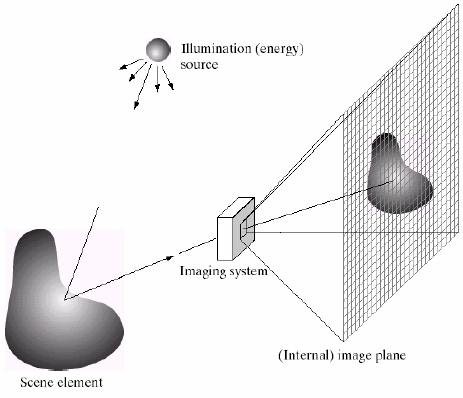
\includegraphics[height=.4\textheight]{./images/img_form.png}
      \end{figure}
      \begin{itemize}\scriptsize
        \item $f(x,y)$: intensity or brightness of a pixel at a position $(x,y)$
        \item $0 < f(x,y) < +\infty$
      \end{itemize}
    \end{block}
\end{frame}

\begin{frame}
  \frametitle{Digital Image}
  %\framesubtitle{}
    \begin{block}{Digital image formation}
        \begin{figure}
        \centering
        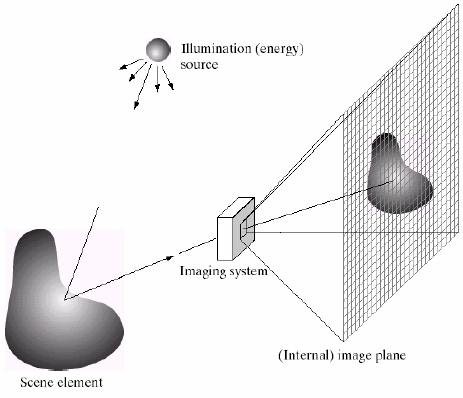
\includegraphics[height=.4\textheight]{./images/img_form.png}
      \end{figure}
      \begin{itemize}\scriptsize
        \item<1-> $r(x,y)$: illumination --- $[0, +\infty[$
        \item<2-> $i(x,y)$: reflectance --- $[0,1]$
        \item<3-> $f(x,y) = r(x,y) i(x,y)$
        \end{itemize}
    \end{block}
\end{frame}

\begin{frame}
  \frametitle{Digital Image}
  %\framesubtitle{}
    \begin{block}{Example of reflectance}
      \begin{itemize}\scriptsize
        \item Black velvet: 0.01
        \item Snow: 0.93
        \end{itemize}
    \end{block}
    \begin{block}{Example of illumination}
      \begin{itemize}\scriptsize
        \item Sunny day: 9000 foot-candles
        \item Cloudy day: 1000 foot-candles
        \item Full moon: 0.01 foot-candles
        \end{itemize}
    \end{block}
\end{frame}

\begin{frame}
  \frametitle{Digital Image}
%   %\framesubtitle{}
    \begin{block}{In practise}
      \begin{itemize}\scriptsize
      \item $i(x,y)$ and $r(x,y)$ are bounded
      \end{itemize}
      {\scriptsize
      \begin{eqnarray}
        i_{\text{min}}(x_0, y_0) r_{\text{min}}(x_0, y_0) < & f(x_0, y_0) & < i_{\text{max}}(x_0, y_0) r_{\text{max}}(x_0, y_0) \ , \\
        L_\text{min} < & f(x_0, y_0) & < L_\text{max} \ .
      \end{eqnarray}}
    \begin{itemize}
      \item $[L_\text{min}, L_\text{max}] \approx [10, 1000]$ --- Shifted in $[0, L-1]$
    \end{itemize}
    \only<2>{
    $\rightarrow$ What is the value for true white and black colors in an image?}
    \end{block}
\end{frame}

\subsection{Sampling \& quantisation}

\begin{frame}
  \frametitle{Digital Image}
%   %\framesubtitle{}
    \only<1>{\begin{block}{Conversion from continuous to digital}
      \begin{itemize}
        \item $f(x,y)$ is a continuous function with regarding the coordinates and the amplitude
        \item Image sampling to refer to spatial coordinates
        \item Signal quantisation to digitise the amplitude 
      \end{itemize}
    \end{block}}
  \only<2>{\begin{block}{Sampling}
        \begin{figure}
        \centering
        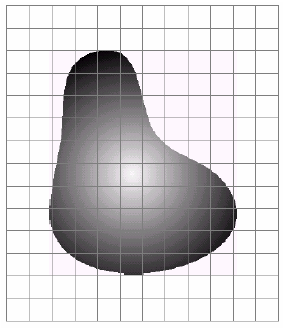
\includegraphics[height=.6\textheight]{./images/sampling.png}
      \end{figure}
    \end{block}}
  \only<3>{\begin{block}{Quantisation}
        \begin{figure}
        \centering
        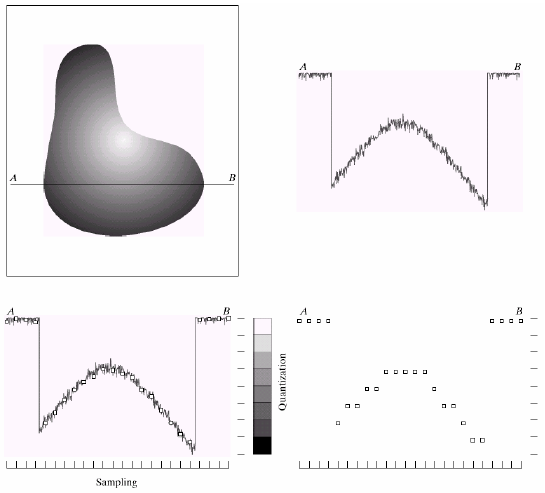
\includegraphics[height=.6\textheight]{./images/quantisation.png}
      \end{figure}
    \end{block}}
  \only<4>{\begin{block}{Digital image}
        \begin{figure}
        \centering
        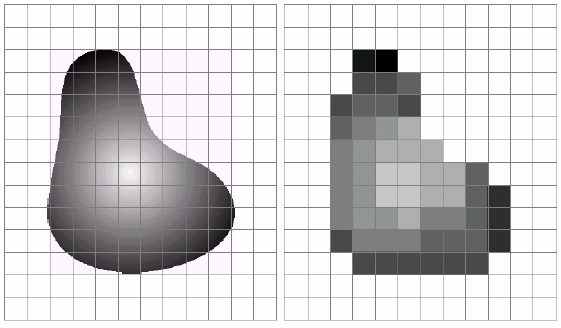
\includegraphics[height=.4\textheight]{./images/dig_img.png}
      \end{figure}
      \begin{itemize}\scriptsize
        \item Check the appendix notebook
      \end{itemize}
    \end{block}}
\end{frame}

\begin{frame}
  \frametitle{Digital Image}
%   %\framesubtitle{}
    \only<1>{\begin{block}{Coordinate system convention}
        \begin{figure}
        \centering
        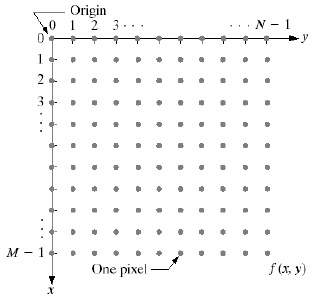
\includegraphics[height=.6\textheight]{./images/coo_img.png}
      \end{figure}
    \end{block}}
\end{frame}

\begin{frame}
  \frametitle{Digital Image}
%   %\framesubtitle{}
    \only<1>{\begin{block}{Digitisation requirements}
        \begin{itemize}\scriptsize
          \item Set an height: $M$
          \item Set an width: $N$
          \item Set an intensity level: $L = 2^k$ and equally spaced
          \item \emph{Dynamic range} : $\frac{L_{\text{min}}}{L_{\text{max}}}$
        \end{itemize}
        \begin{figure}
        \centering
        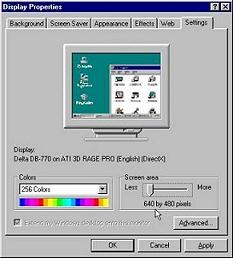
\includegraphics[height=.4\textheight]{./images/windows.jpg}
      \end{figure}
    \end{block}}
\end{frame}

\begin{frame}
  \frametitle{Digital Image}
%   %\framesubtitle{}
    \only<1>{\begin{block}{Parameter variations}
        \begin{figure}
        \centering
        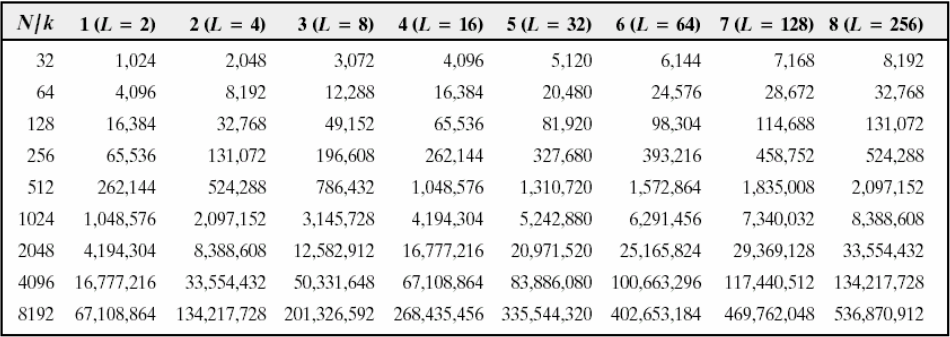
\includegraphics[width=.8\textwidth]{./images/storage.png}
      \end{figure}
      $\rightarrow$ What is the best values regarding the resolution and dynamic range parameters?
      \begin{itemize}\scriptsize
        \item Larger is better ...
        \item ... storage and processing could be a problem
      \end{itemize}
    \end{block}}
\end{frame}

\begin{frame}
  \frametitle{Digital Image}
%   %\framesubtitle{}
    \only<1>{\begin{block}{Isopreference curves}
        \begin{figure}
        \centering
        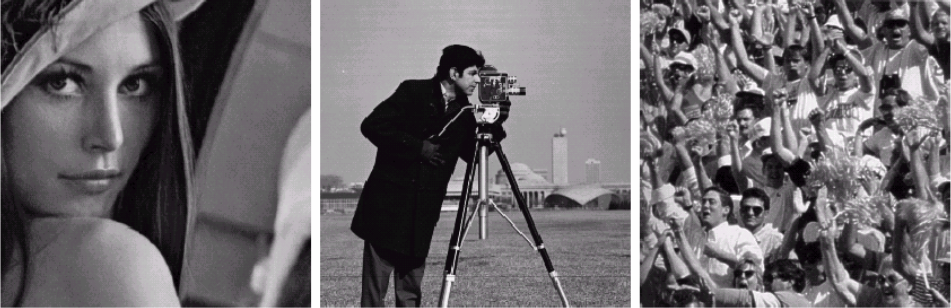
\includegraphics[width=.6\textwidth]{./images/iso1.png}
      \end{figure}
      \vspace{-.7cm}
      \begin{figure}
        \centering
        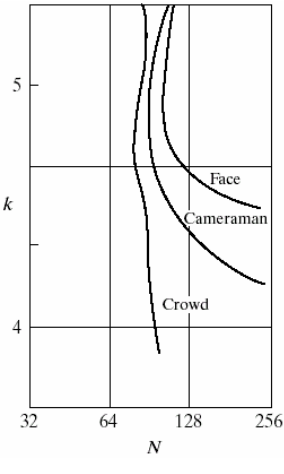
\includegraphics[height=.3\textheight]{./images/iso2.png}
      \end{figure}
    \end{block}}
\end{frame}

\begin{frame}
  \frametitle{Digital Image}
%   %\framesubtitle{}
    \only<1->{\begin{block}{Non-uniform sampling and quantisation}
        \begin{itemize}
          \item<2-> Fine sampling in details region --- coarse sampling in smooth region
          \item<3-> Few gray levels in details regions --- more in smooth region
        \end{itemize}
    \end{block}}
\end{frame}

\section{Pixel Relationships}

\subsection{Neighbours}

\begin{frame}
  \frametitle{Pixel Relationships}
  %   % \framesubtitle{}
  \only<1->{\begin{block}{Neighours}\scriptsize
      \begin{columns}
        \begin{column}{.33\linewidth}
          \begin{center}
            \emph{4-neighbours} --- N\textsubscript{4}-p\\\vspace{.5cm}
            \only<1>{\begin{tabular}{|c|c|c|c|c|}
                \hline
                0 & 1 & 1 & 1 & 0\\ \hline
                0 & 1 & 0 & 0 & 1\\ \hline
                0 & 0 & \cellcolor{azulunam!50}1 & 0 & 0\\ \hline
                1 & 0 & 1 & 1 & 0\\ \hline
                0 & 1 & 1 & 0 & 1\\ \hline
              \end{tabular}}
              \only<2->{\begin{tabular}{|c|c|c|c|c|}
                \hline
                0 & 1 & 1 & 1 & 0\\ \hline
                0 & 1 & \cellcolor{orounam!50}0 & 0 & 1\\ \hline
                0 & \cellcolor{orounam!50}0 & \cellcolor{azulunam!50}1 & \cellcolor{orounam!50}0 & 0\\ \hline
                1 & 0 & \cellcolor{orounam!50}1 & 1 & 0\\ \hline
                0 & 1 & 1 & 0 & 1\\ \hline
              \end{tabular}}
          \end{center}
        \end{column}
        \begin{column}{.33\linewidth}
          \begin{center}
          \emph{D-neighbours} --- N\textsubscript{D}-p\\\vspace{.5cm}
            \only<1-2>{\begin{tabular}{|c|c|c|c|c|}
                \hline
                0 & 1 & 1 & 1 & 0\\ \hline
                0 & 1 & 0 & 0 & 1\\ \hline
                0 & 0 & \cellcolor{azulunam!50}1 & 0 & 0\\ \hline
                1 & 0 & 1 & 1 & 0\\ \hline
                0 & 1 & 1 & 0 & 1\\ \hline
              \end{tabular}}
              \only<3->{\begin{tabular}{|c|c|c|c|c|}
                \hline
                0 & 1 & 1 & 1 & 0\\ \hline
                0 & \cellcolor{orounam!50}1 & 0 & \cellcolor{orounam!50}0 & 1\\ \hline
                0 & 0 & \cellcolor{azulunam!50}1 & 0 & 0\\ \hline
                1 & \cellcolor{orounam!50}0 & 1 & \cellcolor{orounam!50}1 & 0\\ \hline
                0 & 1 & 1 & 0 & 1\\ \hline
              \end{tabular}}
          \end{center}
        \end{column}
        \begin{column}{.33\linewidth}
          \begin{center}
            \emph{8-neighbours} --- N\textsubscript{8}-p\\\vspace{.5cm}
            \only<1-3>{\begin{tabular}{|c|c|c|c|c|}
                \hline
                0 & 1 & 1 & 1 & 0\\ \hline
                0 & 1 & 0 & 0 & 1\\ \hline
                0 & 0 & \cellcolor{azulunam!50}1 & 0 & 0\\ \hline
                1 & 0 & 1 & 1 & 0\\ \hline
                0 & 1 & 1 & 0 & 1\\ \hline
              \end{tabular}}
              \only<4>{\begin{tabular}{|c|c|c|c|c|}
                \hline
                0 & 1 & 1 & 1 & 0\\ \hline
                0 & \cellcolor{orounam!50}1 & \cellcolor{orounam!50}0 & \cellcolor{orounam!50}0 & 1\\ \hline
                0 & \cellcolor{orounam!50}0 & \cellcolor{azulunam!50}1 & \cellcolor{orounam!50}0 & 0\\ \hline
                1 & \cellcolor{orounam!50}0 & \cellcolor{orounam!50}1 & \cellcolor{orounam!50}1 & 0\\ \hline
                0 & 1 & 1 & 0 & 1\\ \hline
              \end{tabular}}
          \end{center}
        \end{column}
      \end{columns}
    \end{block}}
\end{frame}

\subsection{Adjacency}

\begin{frame}
  \frametitle{Pixel Relationships}
  %   % \framesubtitle{}
  \begin{block}{Adjacency}\scriptsize
      \begin{center}
        \vspace{.1cm}
        Let denotes $V=\{1\}$ defining the adjacency
        \vspace{-.3cm}
      \end{center}
      \begin{columns}
        \begin{column}{.33\linewidth}
          \begin{center}
            \emph{4-adjacency}\\\vspace{.5cm}
            \only<1>{\begin{tabular}{|c|c|c|c|c|}
                \hline
                0 & 1 & 1 & 1 & 0\\ \hline
                0 & 1 & 0 & 0 & 1\\ \hline
                0 & 0 & \cellcolor{azulunam!50}1 & 0 & 0\\ \hline
                1 & 0 & 1 & 1 & 0\\ \hline
                0 & 1 & 1 & 0 & 1\\ \hline
              \end{tabular}}
            \only<2->{\begin{tabular}{|c|c|c|c|c|}
                \hline
                0 & 1 & 1 & 1 & 0\\ \hline
                0 & 1 & 0 & 0 & 1\\ \hline
                0 & 0 & \cellcolor{azulunam!50}1 & 0 & 0\\ \hline
                1 & 0 & \cellcolor{orounam!50}1 & 1 & 0\\ \hline
                0 & 1 & 1 & 0 & 1\\ \hline
              \end{tabular}}
          \end{center}
        \end{column}
        \begin{column}{.33\linewidth}
          \begin{center}
            \emph{8-adjacency}\\\vspace{.5cm}
            \only<1-2>{\begin{tabular}{|c|c|c|c|c|}
                \hline
                0 & 1 & 1 & 1 & 0\\ \hline
                0 & 1 & 0 & 0 & 1\\ \hline
                0 & 0 & \cellcolor{azulunam!50}1 & 0 & 0\\ \hline
                1 & 0 & 1 & 1 & 0\\ \hline
                0 & 1 & 1 & 0 & 1\\ \hline
              \end{tabular}}
              \only<3->{\begin{tabular}{|c|c|c|c|c|}
                \hline
                0 & 1 & 1 & 1 & 0\\ \hline
                0 & \cellcolor{orounam!50}1 & 0 & 0 & 1\\ \hline
                0 & 0 & \cellcolor{azulunam!50}1 & 0 & 0\\ \hline
                1 & 0 & \cellcolor{orounam!50}1 & \cellcolor{orounam!50}1 & 0\\ \hline
                0 & 1 & 1 & 0 & 1\\ \hline
              \end{tabular}}
          \end{center}
        \end{column}
        \begin{column}{.33\linewidth}
          \begin{center}
            \emph{m-adjacency}\\\vspace{.5cm}
            \only<1-3>{\begin{tabular}{|c|c|c|c|c|}
                \hline
                0 & 1 & 1 & 1 & 0\\ \hline
                0 & 1 & 0 & 0 & 1\\ \hline
                0 & 0 & \cellcolor{azulunam!50}1 & 0 & 0\\ \hline
                1 & 0 & 1 & 1 & 0\\ \hline
                0 & 1 & 1 & 0 & 1\\ \hline
              \end{tabular}}
              \only<4>{\begin{tabular}{|c|c|c|c|c|}
                \hline
                0 & 1 & 1 & 1 & 0\\ \hline
                0 & 1 & 0 & 0 & 1\\ \hline
                0 & 0 & \cellcolor{azulunam!50}1 & 0 & 0\\ \hline
                1 & 0 & \cellcolor{orounam!50}1 & 1 & 0\\ \hline
                0 & 1 & 1 & 0 & 1\\ \hline
              \end{tabular}
            $q \in N_4(p)$}
          \only<5>{\begin{tabular}{|c|c|c|c|c|}
                \hline
                0 & 1 & 1 & 1 & 0\\ \hline
                0 & \cellcolor{orounam!50}1 & 0 & 0 & 1\\ \hline
                0 & 0 & \cellcolor{azulunam!50}1 & 0 & 0\\ \hline
                1 & 0 & 1 & \cellcolor{orounam!50}1 & 0\\ \hline
                0 & 1 & 1 & 0 & 1\\ \hline
              \end{tabular}
            $q \in N_D(p)$}
          \only<6>{\begin{tabular}{|c|c|c|c|c|}
                \hline
                0 & 1 & 1 & 1 & 0\\ \hline
                0 & \cellcolor{orounam!50}1 & 0 & 0 & 1\\ \hline
                0 & 0 & \cellcolor{azulunam!50}1 & 0 & 0\\ \hline
                1 & 0 & 1 & 1 & 0\\ \hline
                0 & 1 & 1 & 0 & 1\\ \hline
              \end{tabular}
            $q \in N_D(p)$ AND $N_4(p) \cap N_4(q) \notin V$}
          \only<7>{\begin{tabular}{|c|c|c|c|c|}
                \hline
                0 & 1 & 1 & 1 & 0\\ \hline
                0 & \cellcolor{orounam!50}1 & 0 & 0 & 1\\ \hline
                0 & 0 & \cellcolor{azulunam!50}1 & 0 & 0\\ \hline
                1 & 0 & \cellcolor{orounam!50}1 & 1 & 0\\ \hline
                0 & 1 & 1 & 0 & 1\\ \hline
              \end{tabular}}
          \end{center}
        \end{column}
      \end{columns}
    \end{block}
\end{frame}

\subsection{Path}

\begin{frame}
  \frametitle{Pixel Relationships}
  %   % \framesubtitle{}
  \begin{block}{Path}\scriptsize
    \begin{center}
    \only<1>{\begin{tabular}{|c|c|c|c|c|}
      \hline
      0 & \cellcolor{azulunam!50}1 & 1 & 1 & 0\\ \hline
      0 & 1 & 0 & 0 & 1\\ \hline
      0 & 1 & 1 & 0 & 0\\ \hline
      1 & 0 & 1 & 1 & 0\\ \hline
      0 & 1 & 1 & 1 & \cellcolor{azulunam!50}1\\ \hline
    \end{tabular}}
  \only<2>{
    4-path\\\vspace{.7cm}
    \begin{tabular}{|c|c|c|c|c|}
      \hline
      0 & \cellcolor{azulunam!50}1 & 1 & 1 & 0\\ \hline
      0 & \cellcolor{orounam!50}1 & 0 & 0 & 1\\ \hline
      0 & \cellcolor{orounam!50}1 & \cellcolor{orounam!50}1 & 0 & 0\\ \hline
      1 & 0 & \cellcolor{orounam!50}1 & 1 & 0\\ \hline
      0 & 1 & \cellcolor{orounam!50}1 & \cellcolor{orounam!50}1 & \cellcolor{azulunam!50}1\\ \hline
    \end{tabular}}
  \only<3>{
    8-path\\\vspace{.7cm}
    \begin{tabular}{|c|c|c|c|c|}
      \hline
      0 & \cellcolor{azulunam!50}1 & 1 & 1 & 0\\ \hline
      0 & \cellcolor{orounam!50}1 & 0 & 0 & 1\\ \hline
      0 & 1 & \cellcolor{orounam!50}1 & 0 & 0\\ \hline
      1 & 0 & 1 & \cellcolor{orounam!50}1 & 0\\ \hline
      0 & 1 & 1 & 1 & \cellcolor{azulunam!50}1\\ \hline
    \end{tabular}}
    \only<4>{
    m-path\\\vspace{.7cm}
    \begin{tabular}{|c|c|c|c|c|}
      \hline
      0 & \cellcolor{azulunam!50}1 & 1 & 1 & 0\\ \hline
      0 & \cellcolor{orounam!50}1 & 0 & 0 & 1\\ \hline
      0 & \cellcolor{orounam!50}1 & \cellcolor{orounam!50}1 & 0 & 0\\ \hline
      1 & 0 & \cellcolor{orounam!50}1 & 1 & 0\\ \hline
      0 & 1 & \cellcolor{orounam!50}1 & \cellcolor{orounam!50}1 & \cellcolor{azulunam!50}1\\ \hline
    \end{tabular}
  \begin{itemize}
    \item if $(x_{\text{init}}, y_{\text{init}}) = (x_{\text{end}}, y_{\text{end}}) \rightarrow$ closed path 
  \end{itemize}}
  \end{center}
  \end{block}
\end{frame}

\subsection{Subset \& region}

\begin{frame}
  \frametitle{Pixel Relationships}
  %   % \framesubtitle{}
  \begin{block}{Subset}
    \begin{itemize}
    \item $p$ and $q$ are \emph{connected} in the subset $S$ if there is a path in with all the pixels belonging to $S$
    \item For any pixel $p$ in $S$, the set of pixels in $S$ that are connected to p is a \emph{connected component} of $S$
    \item If $S$ has only one connected component then $S$ is called a \emph{connected set}
    \end{itemize}
  \end{block}
  \begin{block}{Region}
    \begin{itemize}
    \item $R$ is a subset of pixels: $R$ is a region if $R$ is a connected set
    \item Region can be \emph{adjacent} or \emph{disjoint}
    \end{itemize}
  \end{block}
\end{frame}

\subsection{Distance measures}

\begin{frame}
  \frametitle{Pixel Relationships}
  \framesubtitle{Distance measures}
  \only<1>{\begin{block}{Definition}
    For pixels $p,q,z$ with coordinates $(x,y)$, $(s,t)$, $(u,v)$, $D$ is a distance function or metric if:
    \begin{itemize}
    \item $D(p,q) \geq 0 \ (D(p,q)=0 \text{ iff } p=q)$
    \item $D(p,q) = D(q,p)$ and
    \item $D(p,z) \leq D(p,q) + D(q,z)$
    \end{itemize}
  \end{block}}
  \only<2>{\begin{block}{Euclidean distance}
    For pixels $p,q,z$ with coordinates $(x,y)$, $(s,t)$, $(u,v)$:
    \begin{itemize}
    \item  $D_e(p,q) = \sqrt{(x-s)^2 + (y-t)^2}$
    \end{itemize}
  \end{block}
  \begin{block}{D\textsubscript{4} distance}
    \begin{itemize}
    \item  $D_4(p,q) = |x-s| + |y-t|$
    \end{itemize}
  \end{block}
  \begin{block}{D\textsubscript{8} distance}
    \begin{itemize}
    \item  $D_8(p,q) = \text{max}(|x-s|, |y-t|)$
    \end{itemize}
  \end{block}
  \begin{block}{D\textsubscript{m} distance}
    \begin{itemize}
    \item  Shortest $m$-path considering the $m$-adjacency
    \end{itemize}
  \end{block}}
\end{frame}

\end{document}